\documentclass[12pt,a4paper]{article}
\linespread{1}
\usepackage[utf8]{inputenc}
\usepackage[margin=1in]{geometry}
\usepackage{amsmath}
\usepackage{amsthm}
\usepackage{amsfonts}
\usepackage{wrapfig,lipsum,booktabs}
\usepackage{ragged2e}
\usepackage{amssymb}
\usepackage[font=footnotesize,labelfont=bf]{caption}
\usepackage{subcaption}
\usepackage[usenames, dvipsnames]{color}
\usepackage{graphicx}
\usepackage{float}
\usepackage{hhline}
\usepackage{tabularx}
\usepackage[citestyle=authoryear, bibstyle=authoryear,backend=biber]{biblatex}
\DeclareUnicodeCharacter{8208}{-}

\newtheorem{theorem}{Theorem}

\newcommand{\rojo}{\textcolor{red}}
\newcommand{\azul}{\textcolor{blue}}

\bibliography{ref.bib}
\title{Outlining a Posterior-Approximating HMCMC Algorithm}

\begin{document}
\maketitle
\section{Brief Intro}
We would like to design an MCMC algorithm that combines Hamiltonian MCMC (HMCMC) \parencite{neal_mcmc_2012,betancourt_geometric_2014,betancourt_conceptual_2017} and the approximate posterior + refinement approach of the Shrinking Bullseye \parencite{conrad_accelerating_2015}. 

The basic skeleton of an HMCMC algorithm procedes as follows:
\begin{enumerate}
\item Consider the sampler at point $\vec{q}_n$ in parameter space with posterior density $\pi(\vec{q} | \vec{y})$ where $\vec{y}$ is the observed data (supressed going forward) .
\item Draw a momentum vector $\vec{p}_n$ from the distribution $\pi(\vec{p} | \vec{q} ) = \text{N}(\vec{p} |0, M)$ where $M$ is the mass matrix (in vanilla HMCMC this is usually chosen to be the covariance matrix of $\pi(\vec{q}|\vec{y})$ but for Riemanian HMCMC I believe one uses the Hessian of $\pi(\vec{q})$ with respect to $\vec{q}$ evaluated at $\vec{q}_n$, or something similar).
\item We then numerically integrate the following Hamiltonian with step size $h$ for $s$ steps (the integration time $sh$ is a free parameter for the sampler, and needs to be chosen wisely based on the geometry of the posterior), with initial conditions $(\vec{q}_n, \vec{p}_n)$:
\begin{equation}
\begin{split}
\dot{\vec{q}} &= M^{-1} \vec{p} \\ 
\dot{\vec{p}} &= - \nabla ln(\pi(\vec{q}))\\
\end{split}
\end{equation}
\item This integration is typically done by the leapfrog method, but any other \textit{symplectic} numerical integrator will work.  This takes the form:
\begin{equation}
\begin{split}
\vec{p}_{t+h/2} &= \vec{p}_t - (\frac{h}{2})  \nabla ln(\pi(\vec{q_t}))\\
\vec{q}_h &= \vec{q}_t + (h)M^{-1} \vec{p}_{t+h/2} \\ 
\vec{p}_h &= \vec{p}_{t+h/2} - (\frac{h}{2})  \nabla ln(\pi(\vec{q_{t+h}})) \\
\end{split}
\end{equation}
\item After integrating to time $sh$ the candidate points $q_{n+1}, p_{n+1}$ (supressing vector notation) are set as $q_{n+sh}, p_{n+sh}$.  To make the process reversible we need to now negate $p_{n+1}$, so our candidate points are $q_{n+1}, -p_{n+1}$.  Then the candidate $q_{n+1}$ gets plugged into the usual Metropolis accept/reject probability.  Doing a Metropolis accept/reject would not be necessary if we could integrate (1) without error, but due to the error in (2) we would get biased estimates without the Metropolis step.
\end{enumerate}

\section{Testing Approximation Methods}
Based on my criteria (see Appendix) and conversation with Ian Grooms (see update from 6/2) I identified two approximating algorithms to compare: (1) Local Quadratic Regression (LQR) and (2) radial basis functions (specifically Thin Plate Splines, TPS).  This are both gridless methods, so are well-suited to ad hoc additions to the approximating set $S$.  Here I implement both and compare their performance (the TPS was implemented with no low-rank approximation, as it reduced approximation quality substantially without providing a substantial computational speedup).

For comparison of performance I used the test density function:
\begin{equation}
\pi(x,y) = \text{Exp} \left( -P*(A*x^2*y^2 + x^2 + y^2 - B*x*y - C*x - C*y) \right)
\end{equation}
With $A = C = 1$, $ B =10$ and $ P = 0.05$ (Fig. 1).  For gradient calculations I used the NumPy \texttt{gradient()} function, which computes the gradient by central differences.  It should be noted that for both LQR and TPS the gradient can be computed by hand, but it was simpler in implementation to just use central differences for now.  To compare the methods I fit them with 300 points chosen uniformly over the square $[-15,15] \times [-15,15]$ and computed the gradient at 1e5 gridpoints over the square $[-6,6] \times [-6,6]$.  Letting $\hat{\pi}_i$ denote the approximation from method $i$, I computed the max gradient error as:
\[
\epsilon_i = \frac{ \text{max}_{j} \left( \Vert \nabla \hat{\pi}_i(\vec{x}^{(j)}) - \nabla \pi(\vec{x}^{(j)})  \Vert \right) } { \text{max}_j \left( \Vert \nabla \pi(\vec{x}^{(j)}) \Vert \right) }
\]
Where the max's are taken over the grid points $\vec{x}^{(j)}$. I similarly computing a max function error:
\[
e_i = \frac{ \text{max}_{j} \left( \Vert \hat{\pi}_i(\vec{x}^{(j)}) - \pi(\vec{x}^{(j)})  \Vert \right) } { \text{max}_j \left( \Vert \pi(\vec{x}^{(j)}) \Vert \right) }
\]

The thin plate splines fared substantially better, with $e_{\text{TPS}} = 0.319$ and $\epsilon_{\text{TPS}} = 0.826$ compared to $e_{\text{LQR}} = 0.596$ and $\epsilon_{LQR} = 57.9$.  This was calculated with a TPS smoothness parameter $\lambda = 1e-7$.  To asses how varying this parameter changed the TPS fit I re-computed $e_{\text{TPS}}$ and $\epsilon_{\text{TPS}}$ for each $\lambda \in [1e-10, 1e-7,1e-4, 1e-1, 1, 10, 100]$.

\begin{figure}
\centering
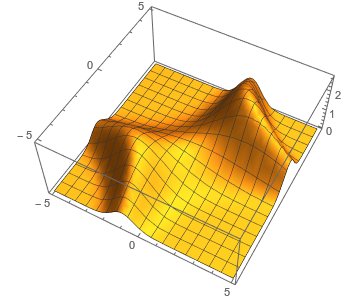
\includegraphics[scale=.6]{./Figs/test_dense.png}
\caption{The test density function in (3) with $A = 1, B =10, C = 1, P = 0.05$}
\end{figure}

\section{Goals for Next Week}
\begin{itemize}
\item Diagnose and fix RBF interpolation scheme (may have to get back in touch with Ian for help with this)
\item Add Greg's changes to the variance reduction paper, meet with him again on Friday to discuss them.
\end{itemize}

\section{Appendix: Approximation Criteria}
The key feature in the Shrinking Bullseye is the inclusion of the refinements to the set of samples $S$ and $\pi(S)$ used for approximating the posterior density $\pi()$.  Thinking about adapting their basic scheme (including the refinements) to HMCMC I identified the following criteria that an approximation method for $\pi()$ should satisfy to be a good candidate for the algorithm:
\begin{enumerate}
\item The approximation must be good for both $\pi$ and $\nabla \pi$, and our interpolant must be at least once differentiable anywhere in the support of $\pi$ (twice if we’d like to do Riemanian HMCMC). Furthermore it must be straightforward or cheap to evaluate $\nabla \pi$ since we have to do so twice during a single evaulation of (2), and we are performing $s$ such evaluations per step of the sampler so total that’s $2s$ gradient evaluations per candidate proposal.
\item The approximation has to be amenable to refinements. Whatever interpolation scheme  we use, it must allow us to test for refinements (ideally through something like the cross-validation approach in the Shrinking Bullseye) as well as add new points to the interpolating data set on an ad hoc basis (ie. whenever and wherever the refinement criteria is triggered).
\item  The Hamiltonian dynamics induced by the approximation  need to be similar enough to $\pi$ that the candidates proposed are actually good. Following Betancourt’s “Conceptual Introduction to Hamiltonian Monte Carlo”, our interpolant needs to approximate the true posterior well on its typical set.
\end{enumerate}

\printbibliography

\end{document}


%%% Local Variables:
%%% mode: latex
%%% TeX-master: t
%%% End:
